\documentclass[tikz,border=6pt]{standalone}
\usepackage{xcolor}
\usetikzlibrary{arrows.meta}
\tikzset{
  actor/.style={draw, rounded corners, fill=orange!12, minimum width=3.0cm, minimum height=0.85cm, align=center, font=\small},
  msg/.style={->, >=Latex, thick},
  lane/.style={gray!60, dashed}
}
\begin{document}
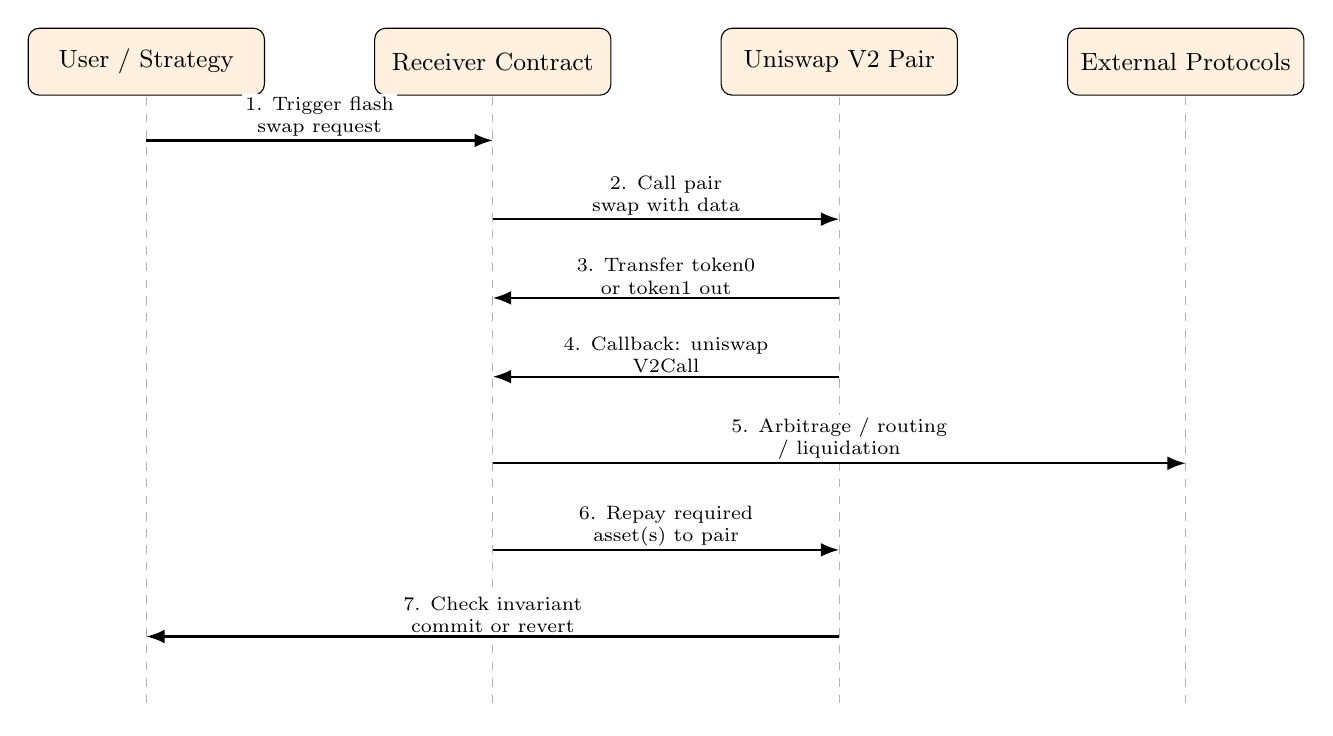
\begin{tikzpicture}[x=1cm,y=1cm]
  \node[actor] at (0,0) {User / Strategy};
  \node[actor] at (4.4,0) {Receiver Contract};
  \node[actor] at (8.8,0) {Uniswap V2 Pair};
  \node[actor] at (13.2,0) {External Protocols};

  \draw[lane] (0,-0.45) -- (0,-8.2);
  \draw[lane] (4.4,-0.45) -- (4.4,-8.2);
  \draw[lane] (8.8,-0.45) -- (8.8,-8.2);
  \draw[lane] (13.2,-0.45) -- (13.2,-8.2);

  \draw[msg] (0,-1.0) -- node[midway, above, fill=white, inner sep=1pt, font=\scriptsize, align=center]{1. Trigger flash\\swap request} (4.4,-1.0);
  \draw[msg] (4.4,-2.0) -- node[midway, above, fill=white, inner sep=1pt, font=\scriptsize, align=center]{2. Call pair\\swap with data} (8.8,-2.0);
  \draw[msg] (8.8,-3.0) -- node[midway, above, fill=white, inner sep=1pt, font=\scriptsize, align=center]{3. Transfer token0\\or token1 out} (4.4,-3.0);
  \draw[msg] (8.8,-4.0) -- node[midway, above, fill=white, inner sep=1pt, font=\scriptsize, align=center]{4. Callback: uniswap\\V2Call} (4.4,-4.0);
  \draw[msg] (4.4,-5.1) -- node[midway, above, fill=white, inner sep=1pt, font=\scriptsize, align=center]{5. Arbitrage / routing\\/ liquidation} (13.2,-5.1);
  \draw[msg] (4.4,-6.2) -- node[midway, above, fill=white, inner sep=1pt, font=\scriptsize, align=center]{6. Repay required\\asset(s) to pair} (8.8,-6.2);
  \draw[msg] (8.8,-7.3) -- node[midway, above, fill=white, inner sep=1pt, font=\scriptsize, align=center]{7. Check invariant\\commit or revert} (0,-7.3);
\end{tikzpicture}
\end{document}
